\chapter{LANDASAN TEORI}

 \section{Python}
	 Python adalah bahasa pemrograman interpretatif multiguna dengan prinsip agar sumber kode yang dihasilkan memiliki tingkat keterbacaan yang baik. Python diklaim sebagai bahasa yang menggabungkan kapabilitas, kemampuan, dengan sintaksis kode yang sangat jelas, dan dilengkapi dengan fungsionalitas pustaka standar yang besar serta komprehensif. Python mendukung beragam paradigma pemrograman, seperti pemrograman berorientasi objek, pemrograman imperatif, dan pemrograman fungsional. Python dapat digunakan untuk berbagai keperluan pengembangan perangkat lunak dan dapat berjalan di berbagai platform sistem operasi \cite{bab2-python} \\

 \section{Flask}
	 Flask adalah sebuah kerangka kerja web. Artinya, Flask menyediakan perangkat, pustaka, dan teknologi yang memungkinkan seorang pengembang untuk membangun aplikasi berbasis web. Aplikasi web yang bisa dibangun bisa berupa sebuah halaman web, blog, wiki, bahkan untuk web komersial. Flask dibangun berbasiskan pada Werkzeug, Jinja 2, dan MarkupSafe yang mana menggunakan bahasa pemrograman Python sebagai basisnya. Flask sendiri pertama kali dikembangkan pada tahun 2010 dan didistribusikan dengan lisensi BSD \\
	 \indent Flask termasuk sebagai perangkat kerja mikro karena tidak membutuhkan banyak perangkat atau pustaka tertentu agar bisa bekerja. Flask tidak menyediakan fungsi untuk melakukan interaksi dengan basis data, tidak mempunya validasi \textit{form} atau fungsi lain yang umumnya bisa digunakan dan disediakan pada sebuah kerangka kerja web. Meskipun memiliki kemampuan yang minim, tapi Flask mendukung dan memberikan kemudahan bagi pengembang untuk menambahkan pustaka sendiri untuk mendukung aplikasinya. Berbagai pustaka seperti validasi \textit{form}, mengunggah file, berbagai macam teknologi autentifikasi bisa digunakan dan tersedia untuk Flask. Bahkan pustaka-pustaka pendukung tersebut lebih sering diperbarui dibandingkan dengan Flasknya sendiri.
	 
 \section{\textit{Gunicorn}}
 \textit{Gunicorn} atau '\textit{Green Unicorn}' adalah \textit{Python} WSGI HTTP \textit{Server} untuk UNIX. Fungsi dari \textit{Gunicorn} ini adalah sebagai pelayan sebuah aplikasi atau sebagai server dari sebuah perangkat lunak yang dikembangkan oleh pengembang.
 
 \textit{Gunicorn} sendiri merupakan salah satu dari sekian banyak \textit{WSGI Server}. Keunggulan dari \textit{Gunicorn} sendiri adalah, \textit{Gunicorn} mampu menangani atau kompatibel dengan berbagai macam kerangka kerja web, sangat mudah untuk diimplementasikan, hanya membutuhkan sedikit sumber daya dari \textit{server} yang terpasang \textit{Gunicorn}, dan juga kerja dari \textit{Gunicorn} yang sangat cepat.
 
 \textit{Gunicorn} mengimplementasikan spesifikasi standar \textit{server WSGI PEP3333} sehingga dapat menjalankan perangkat lunak berbasis \textit{web} yang dikembangkan dengan bahasa pemrograman \textit{python}. Sebagai contoh, perangkat lunak berbasis web yang digunakan oleh penulis menggunakan kerangka kerja \textit{flask}, maka \textit{Gunicorn} dapat menanganinya.
 
 \section{\textit{Supervisor}}
 \textit{Supervisor} adalah sistem yang berbasis \textit{client} atau server, yang memungkinkan penggunanya utuk memantau dan juga mengontrol sejumlah proses pada sistem operasi untuk UNIX. Beberapa faktor terbentuknya \textit{supervisor} antara lain adalah, kenyamanan, ketepatan, delegasi, dan proses grup dalam menggunakan perangkat lunak \textit{supervisor}. Beberapa keunggulan dari perangkat lunak \textit{supervisor} antara lain, konfigurasi yang sederhana, proses yang terpusat, efisien, dapat diperluas penggunaannya, dan juga kompatibel dengan berbagai macam sistem operasi. Komponen dari \textit{supervisor} terbagi menjadi dua, antara lain sebagai berikut.
 
 \subsection{\textit{Supervisord}}
 \textit{Supervisord} merupakan bagian dari \textit{supervisor} yang bertanggung jawab untuk memulai \textit{child programs} atas permintaannya sendiri, menanggapi perintah dari \textit{client}, melakukan \textit{restart} secara otomatis ketika terjadi kerusakan pada proses, mencatat bagian dari proses \texttt{stdout} dan \texttt{stderr} \textit{output}, juga menghasilan dan menangani \textit{events} yang berhubungan dengan bagian-bagian yang digunakan selama \textit{subprocess} tersebut berjalan.
 
 \subsection{\textit{Supervisorctl}}
 \textit{Supervisorctl} merupakan bagian dari \textit{command-line} yang digunakan oleh \textit{client}. \textit{Supervisorctl} menyediakan antarmuka yang mirip dengan fitur \textit{shell} yang disediakan oleh \textit{supervisord}. Dari \textit{supervisorctl}, pengguna dapat terhubung dengan proses \textit{supervisord} yang berbeda satu per satu, mendapatkan status dari \textit{subprocess} yang telah dikontrol, menghentikan atau memulai \textit{subprocess} yang telah dikontrol, dan juga mendapatkan semua daftar proses yang berjalan pada \textit{supervisord}.
 
 \textit{Command-line} dari \textit{client} berhubungan ke \textit{server} melalui \textit{socket domain} UNIX atau melalui \textit{socker internet} (TCP). \textit{Server} dapat menyatakan bahwa \textit{client} harus memberikan \textit{autentifikasi} sebelum mengizinkannya untuk melakukan sebuah perintah. Proses \textit{client} biasanya menggunakan \textit{file} konfigurasi yang sama dengan \textit{server}. 
 
 \section{\textit{Nginx}}
 Nginx adalah sebuah perangkat lunak yang bisa digunakan untuk \textit{web server}, \textit{load balancer}, dan \textit{reverse proxy}. Nginx terkenal karena stabil, memiliki tingkat performa tinggi dan konsumsi sumber daya yang minim. Pada kasus saat terjadi koneksi dalam jumlah yang banyak secara bersamaan, penggunaan \textit{memory}, CPU, dan sumber daya sistem yang lain sangat kecil dan stabil. \cite{chi_web_2012}\\
 \indent Nginx bisa digunakan untuk menyajikan kontent HTTP yang dinamis menggunakan FastCGI, SCGI untuk menangani scripts, aplikasi WSGI , dan bisa juga digunakan sebagai sebuah \textit{load balancer}. Nginx menggunakan \textit{asynchronous event-driven} untuk menangani permintaan. Dengan menggunakan model ini bisa, pengembang bisa melakukan predeksi kinerja Nginx saat terjadi jumlah permintaan yang banyak.
	 
 \section{\textit{Iptables}} 
 \textit{Firewall} merupakan sebuah mekanisme wajib \textit{access} kontrol antar jaringan ataupun antar sistem. \textit{Firewall} ini sangat penting karena bertujuan untuk memastikan keamanan dari sebuah jaringan. \textit{Firewall} dapat menjadi \textit{filter} yang sangat sederhana dan mudah digunakan, tetapi \textit{firewall} juga dapat menjadi \textit{filter} yang sangat penting bagi sebuah jalan keluar suatu jaringan. Prinsip dari penggunaan \textit{firewall} tetaplah sama, dimana penggunaannya untuk \textit{monitoring} dan \textit{filtering} semua pertukaran informasi di jaringan \textit{internal} dan juga di jaringan \textit{external}.
 
 \textit{Netfilter} / \textit{iptables} merupakan sebuah sistem \textit{firewall} berbasis linux yang mempunyai fungsi yang sangat berguna. \textit{Netfilter} / \textit{iptables kernel} menggunakan sebuah mekanisme baru, bernama \textit{iptables}. \textit{Ipbtales} sendiri merupakan sebuah perangkat lunak atau alat yang dapat melakukan manajemen \textit{filter} dari sebuah paket yang ada pada suatu \textit{kernel}. \textit{Iptables} mempunyai \textit{table} dan juga \textit{chain} dari masing-masing \textit{table}. \textit{Table} pada \textit{iptables} terdiri dari tiga, atau juga bisa disebut \textit{iptables} memiliki tiga fungsi utama, antara lain menjadi penyaring paket, mentranslasikan suatu alamat, dan melakuakn penghalusan paket seperti TTL, TOS, dan MARK.
 
 \textit{Filter table} merupakan sebuah konfigurasi \textit{default} dari \textit{iptables}, dimana pada \textit{filter table} terdapat tiga \textit{chain}, antara lain \textit{chain} INPUT, FORWARD, dan OUTPUT. \textit{NAT table} berfungsi untuk merubah tujuan dari sumber dari sebuah paket. Pada \textit{NAT table} terdapat dua \textit{chain}, antara lain \textit{chain} PREROUTING dan POSTROUTING. \textit{Mangle table} berfungsi untuk menghaluskan paket atau juga dapat mengubah isi dari sebuah data kecuali IP \textit{address} dan \textit{port address}.Pada \textit{mangle table} terdapat dua \textit{chain}, antara lain POSTROUTING dan OUTPUT.
	 
 \section{MySQL}
	 MySQL adalah sebuah perangkat lunak terbuka untuk melakukan manajemen basis data SQL atau DBMS. MySQL ditulis dalam bahasa pemrograman C dan C++. MySQL merupakan salah satu perangkat lunak terbuka yang banyak disukai oleh pengembang dan digunakan dalam banyak aplikasi web. Parser SQL yang digunakan ditulis dalam bahasa pemrograman yacc. MySQL bekerja pada banyak \textit{platform}, seperti  FreeBSD, HP-UX, Linux, macOS, Microsoft Windows, NetBSD, OpenBSD, OpenSolaris, Oracle Solaris, dan SunOS. MySQL tersedia sebagai perangkat lunak gratis di bawah lesensi \textit{GNU General Public License} (GPL), tetapi juga tersedia lisensi komersial untuk kasus-kasus dimana penggunanya tidak cocok dengan penggunaan GPL.\\
	 \indent Setiap pengguna dapat secara bebas menggunakan MySQL, namun dengan batasan perangkat lunak tersebut tidak boleh dijadikan produk turunan yang bersifat komersial. MySQL sebenarnya merupakan turunan salah satu konsep utama dalam basis data yang telah ada sebelumnya, yaitu SQL (\textit{Structured Query Language}). SQL adalah sebuah konsep pengoperasian basis data, terutama untuk proses pemilihan atau seleksi dan pemasukan data, yang memungkinkan pengoperasian data dikerjakan dengan mudah.\\
	 \indent Kehandalan suatu sistem basis data dapat diketahui dari cara kerja pengoptimasiannya dalam melakukan proses perintah-perintah SQL yang dibuat oleh pengguna maupun program-program aplikasi yang memanfaatkannya. Sebagai \textit{server} basis data, MySQL mendukung operasi basis data transaksional maupun operasi basis data non-transaksional. Pada modus operasi non-transaksional, MySQL dapat dikatakan handal dalam hal unjuk kerja dibandingkan \textit{server} basis data kompetitor lainnya. Namun pada modus non-transaksional tidak ada jaminan atas reliabilitas terhadap data yang tersimpan, karenanya modus non-transaksional hanya cocok untuk jenis aplikasi yang tidak membutuhkan reliabilitas data seperti aplikasi blogging berbasis web (wordpress), CMS, dan sejenisnya. Untuk kebutuhan sistem yang ditujukan untuk bisnis sangat disarankan untuk menggunakan modus basis data transaksional, hanya saja sebagai konsekuensinya unjuk kerja MySQL pada modus transaksional tidak secepat unjuk kerja pada modus non-transaksional.
	
	\section{\textit{Mitmproxy}}
	
	\textit{Mitmproxy} adalah sebuah sebuah \textit{interception proxy} untuk HTTP dengan antarmuka pengguna \textit{console} yang ditulis dengan bahasa \textit{Python}. \textit{Mitmproxy} merupakan sebuah perangkat lunak yang interaktif dimana \textit{Mitmproxy} memungkinkan dapat memotong dan memodifikasi HTTP \textit{requests} atau \textit{response} dengan sangat cepat.
	
	\textit{Mitmproxy} ada sebuah \textit{proxy} berkemampuan SSL yang berfungsi sebagai \textit{man-in-the-middle} untuk komunikasi HTTP dan HTTPS. Untuk dapat mengetahui atau memodifikasi komunikasi HTTPS, \textit{mitmproxy} berupra-pura menjadi \textit{server} ke \textit{client} dan \textit{client} ke server, sementara itu \textit{mitmproxy} diposisikan di tengah-tengah berfungsi untuk menerjemahkan lalu lintas dari keduanya. \textit{Mitmproxy} menghasilkan sertifikat \textit{on-the-fly} untuk mengetahui \textit{client} agar percaya bahwa mereka berkomunikasi dengan \textit{server}.
	
	Pertama kali \textit{mitmproxy} dimulai, maka akan menghasilkan sertifikat SSL yang berada pada \texttt{~/.mitmproxy/cert.pem}. Sertifikat ini akan digunakan untuk \textit{browser-side}. Karena tidak akan cocok dengan \textit{domain} yang \textit{client} kunjungi, dan tidak akan memverifikasi terhadap otoritas sertifikasi, \textit{client} harus menambahkan pengecualian untuk setiap situs yang \textit{client} kunjungi. Permintaan SSL dicegat dengan hanya mengamsumsikan bahwa semua permintaan \texttt{CONNECT} adalah HTTPS. Sambungan dari \textit{browser} dibungkus SSL, dan kita membaca permintaan dengan berpura-pura menjadi \textit{server} yang menghubungkan.
	
	\section{\textit{VirtualBox}}
	\textit{VirtuaBox} merupakan salah satu produk perangkat lunak yang sekarang dikembangkan oleh Oracle. Aplikasi ini pertama kali dikembangkan oleh perusahaan Jerman, Innotek GmbH. Februari 2008, Innotek GmbH diakusisi oleh Sun Micorsystems. Sun Microsystems kemudian juga diakuisisi oleh Oracle. \textit{VirtualBox} berfungsi untuk melakukan virtualisasi sistem operasi. \textit{VirtualBox} juga dapat digunakan untuk membuat virtualisasi jaringan komputer sederhana. Penggunaan \textit{VirtualBox} ditargetkan untuk \textit{server}, desktop, dan penggunaan \textit{embedded}.
	
	Berdasarkan jenis VMM yang ada, \textit{VirtualBox} merpakan jenis \textit{hypervisor type 2}. \textit{VirtualBox} sendiri memiliki berbagai macam kegunaan, diantaranya \textit{VirtualBox} dapat memainkan semua sistem  operasi baik itu menggunakan windows, linux, atau turunan linux lainnya. \textit{VirtualBox} juga dapat dipergunakan untuk mengujicoba OS baru. \textit{VirtualBox} juga dapat digunakan sebgai media untuk membaut simulasi jaringan.
	
	\section{\textit{Framework} Laravel}
	
	Laravel adalah sebuah \textit{framework} PHP yang dibangun dengan konsep MVC (\textit{Model View Controller}). MVC adalah sebuah pendekatan perangkat lunak yang memisahkan aplikasi logika dari presentasi. MVC memisahkan aplikasi berdasarkan komponen-komponen aplikasi, seperti: manipulasi data, \textit{controller}, dan \textit{user interface}.
	\begin{enumerate}
	\item \textit{Model} berisi fungsi-fungsi yang membantu seseorang dalam pengelolaan data, dan lain-lain.
	\item \textit{View} adalah bagian yang mengatur tampilan ke pengguna. Bisa dikatakan berupa halaman web.
	\item \textit{Controller} merupakan bagian yang menjembatani \textit{model} dan \textit{view}.
	\end{enumerate}
	Rancang Bangun Perangkat Lunak Internet \textit{Access Management} Berbasis Kontainer
	Dalam pembangunan perangkat lunak internet \textit{access management} berbasis kontainer, Laravel digunakan sebagai \textit{framework} untuk pembangunan web sebagai halaman \textit{administrator}. Salah satu fitur yang mendukung proses pengembangan dari Laravel adalah Eloquent ORM. Misalkan, dibutuhkan untuk mengambil semua data yang ada pada tabel \texttt{Kontainer}, maka yang perlu dilakukan hanya membuat sebuah \textit{class model} bernama \textit{Kontainer}. Laravel sendiri dikembangkan secara khusus untuk PHP 7.0. Jadi \textit{framework} ini bisa memanfaatkan berbagai macam kelebihan yang dimiliki PHP versi terbaru tersebut. Tidak ada \textit{backward compatibility} dengan PHP versi sebelumnya.
	
		
	\section{\textit{Docker}}
	Docker adalah sebuah aplikasi yang bersifat \textit{open source} yang berfungsi sebagai wadah untuk memasukkan sebuah perangkat lunak secara lengkap beserta semua hal yang dibutuhkan oelh perangkat lunak tersebut agar dapat berfungsi sebagaimana mestinya. \textit{Docker} dapat dijalankan di berbagai sistem operasi, pengembang dapat dengan mudah menggunakan layanan \textit{docker} melalui \texttt{https://hub.docker.com} untuk mengunduh \textit{imaes} ataupun membuat \textit{images} yang diinginkan. Perbedaan antara \textit{docker} dan \textit{virtual machine} ditunjukkan pada gambar \ref{contohDocker}
	
	\begin{figure}[H] % h = pasti berada di bawah teks yang ada di atas
	\centering
	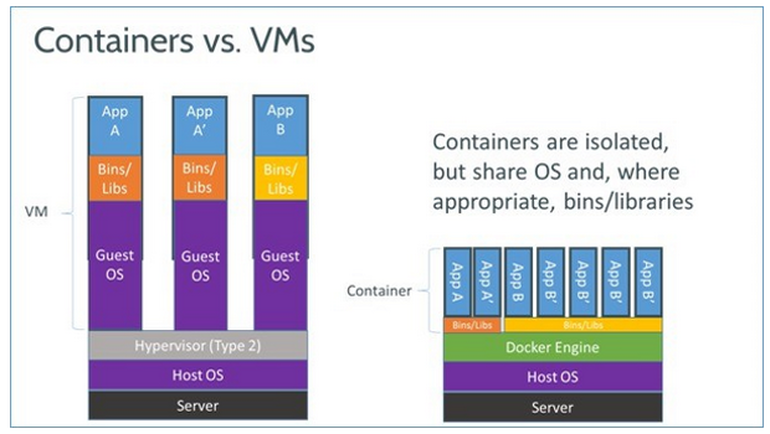
\includegraphics[width=\linewidth]{images/bab2/docker-vm-container}
	\caption{Perbandingan \textit{docker} dan virtual machine}
	\label{contohDocker}
	\end{figure}
	
	\subsection{\textit{Docker Container}}
	\textit{Docker container} atau kontainer \textit{docker} bisa dikatakan sebagai sebuah wadah atau tempat, dimana kontainer \textit{docker} ini dibuat dengan menggunakan \textit{docker image}. Saat kontainer \textit{docker} dijalankan, maka akan terbentu sebuah \textit{layer} di atas \textit{docker image}.Contohnya saat menggunakan \textit{image} Ubuntu, kemudian membuat sebuah kontainer \textit{docker} dari \textit{image} Ubuntu tersebut dengan nama mitmproxy-ubuntu. Setelah itu dilakukan pemasangan sebuah perangkat lunak, misalnya \textit{mitmproxy}, maka secara otomatis kontainer \textit{docker} mitmproxy-ubuntu akan berada di atas \textit{layer image} Ubuntu, dan diatasnya lagi merupakan \textit{layer mitmproxy} berada. \textit{Docker Kontainer} atau Kontainer \textit{docker} ke depannya dapat digunakan untuk menghasilkan sebuah \textit{docker images}. \textit{Docker images} yang dihasilkan dari kontainer \textit{docker} itu sendiri nantinya dapat digunakan kembali untuk membuat kontainer \textit{docker} yang lainnya.
	
	\subsection{\textit{Docker Images}}
	\textit{Docker images} adalah sebuah \textit{blueprint} atau rancangan dasar dari sebuah perangkat lunak berbasis \textit{docker} yang bersifat \textit{read-only}. \textit{Blueprint} ini sendiri merpakan sebuah sistem operasi atau sistem operasi yang telah dipasang berbagai perangkat lunak dan pustaka pendukung. \textit{Docker iamges} berfungsi untuk membuat kontainer \textit{docker}, dimana dengan menggunakan satu \textit{docker iamge} dapat dibuat lebih dari satu kontainer \textit{docker}. \textit{Docker image} sendiri dapat menyelesaikan permasalahan yang dikenal dengan "\textit{dependency hell}", dimana sulitnya untuk melengkapi dependensi sebuah perangkat lunak. Permasalahan tersebut dapat diselesaikan karena semua kebutuhan perangkat lunak sudah berada di dalamnya.
	
	\subsection{\textit{Docker Registry}}
	\textit{Docker Registry} adalah kumpulan dari berbagai macam \textit{docker image} yang bersifat tertutup maupun terbuka yang dapat diakses di \texttt{https://hub.docker.com/} atau dapat diakses pada \textit{server} sendiri. Dengan menggunakan \textit{docker registry}, seseorang dapat menggunakan \textit{docker image} yang telah dibuat oleh orang lainnya. Hal seperti ini dapat mempermudah seseorang untuk melakukan pengembangan dan jugatransfer aplikasi.
	